\documentclass[12pt]{extarticle}
\usepackage{amsmath, amsthm, latexsym, tikz, graphicx, listings, microtype, mathtools, soul, color, fancyhdr}
\usepackage[margin=1in]{geometry}

\newenvironment{myindentpar}[1]%
 {\begin{list}{}%
         {\setlength{\leftmargin}{#1}}%
         \item[]%
 }
 {\end{list}}
 
\DeclarePairedDelimiter\abs{\lvert}{\rvert}%
\DeclarePairedDelimiter\norm{\lVert}{\rVert}%

% Swap the definition of \abs* and \norm*, so that \abs
% and \norm resizes the size of the brackets, and the 
% starred version does not.
\makeatletter
\let\oldabs\abs
\def\abs{\@ifstar{\oldabs}{\oldabs*}}
%
\let\oldnorm\norm
\def\norm{\@ifstar{\oldnorm}{\oldnorm*}}
\makeatother

\definecolor{lightgray}{gray}{0.65}
\definecolor{pinegreen}{RGB}{1, 171, 161}
\definecolor{lightblue}{RGB}{135, 206, 250}
\definecolor{dkgreen}{rgb}{0,0.6,0}
\definecolor{gray}{rgb}{0.5,0.5,0.5}
\definecolor{mauve}{rgb}{0.58,0,0.82}
\definecolor{darkblue}{rgb}{0.0,0.0,0.6}
\definecolor{cyan}{rgb}{0.0,0.6,0.6}

\newcommand*{\Value}{\frac{1}{2}x^2}%
\newcommand{\hlc}[2][yellow]{ {\sethlcolor{#1} \hl{#2}} }

\definecolor{codegray}{gray}{0.9}
\newcommand{\code}[1]{\colorbox{codegray}{\texttt{#1}}}

% /*--------------------------------------------------------------*/
%   Changing the values here sets the due date for the assignment!
% /*--------------------------------------------------------------*/
\newcommand{\duedate}{XX/XX/XX }
\newcommand{\semester}{SEMESTER}

\lstset{frame=tb,
  language=C++,
  breaklines=true,
  showstringspaces=false,
  columns=flexible,
  numbers=none,
  tabsize=3,
  escapeinside={(*@}{@*)}
  %,
  %commentstyle=\color{dkgreen},
  %stringstyle=\color{mauve}
}
\pagestyle{fancy}
\fancyhf{}
\renewcommand{\headrulewidth}{0pt}
\lhead{\color{lightgray} CSCE-313}
\rhead{\color{lightgray} \semester}
\rfoot{\thepage}
\pagenumbering{arabic}

\begin{document}

\begin{center}
    \underline{{\large Machine Problem 4: UNIX Processes \  }(Due: \duedate)}  \\
\end{center}


\ \\
{\large \underline{Introduction}:}

\ \\
The /proc directory is a pseudo filesystem that allows access to kernel data structures while in user space. It allows you to view some of the information the kernel keeps on running processes. To view information about a specific process you just need to view files inside of the directory: /proc/[pid]. For more information simply view the manpage with man proc.  

\ \\
{\large \textbf{The Assignment}:} \newline
\ \\
Using the files stored at /proc write a program/script to find information about a specific process using a user provided pid. In the following, you will find a list of the task\_struct members for which you are required to find their value. In the task\_struct a lot of the data you are finding is not represented as member values but instead pointers to other linux data structures that contain these members. All of the information you will be retrieving can be found in a process’s proc directory (/proc/[pid]).  Your program must be able to retrieve the following data about any given process:  


\begin{center}
    \textbf{Table \#1: Process Attributes}
\end{center}
\begin{displaymath}
    \begin{array}{|l|l|l|}
    \hline
    \text{Category} & \text{Required Variables/Items} & \text{Description} \\ 
    \hline
        \text{Identifiers} & \text{PID, PPID}    & \text{Process ID of the current process and its parent} \\
        \hspace{1cm}       & \text{EUID, EGID}   & \text{Effective user and group ID} \\
        \hspace{1cm}       & \text{RUID, RGID}   & \text{Real user and group ID} \\
        \hspace{1cm}       & \text{FSUID, FSGID} & \text{File system user and group ID} \\
    \hline
        \text{State}       & \text{R, S, D, T, Z, X} & \text{Running, Sleeping, Disk sleeping, Stopped,} \\ \hspace{1cm}       & \hspace{1cm}            & \text{Zombie, and Dead} \\
    \hline
        \text{Thread }     & \text{Thread\_Info} & \text{Thread IDs of a process} \\
        \text{Information} & \hspace{1cm}        & \hspace{1cm}\\
    \hline
        \text{Priority}    & \text{Priority Number} & \text{Integer value from 1 to 99} \\
        \hspace{1cm}       & \text{Niceness Value}  & \text{Integer value from -20 to 19} \\
    \hline
        \text{Time}        & \text{stime \& utime}  & \text{Time that a process has been scheduled} \\
        \text{Information} & \hspace{1cm}           & \text{in kernel/user mode} \\
        \hspace{1cm}       & \text{cstime \& cutime} & \text{Time that a process has waited on children}\\
        \hspace{1cm}       & \hspace{1cm}            & \text{being run in kernel/user mode} \\
    \hline
        \text{Address} & \text{Startcode \& Endcode} & \text{The start and end of a process} \\
        \text{Space}   & \text{ESP \& EIP}           & \text{in memory} \\
    \hline
        \text{Resources} & \text{File Handles \&} & \text{Number of fds used, and number of} \\
        \hspace{1cm}     & \text{Context Switches} & \text{voluntary/involuntary context switches} \\
    \hline
        \text{Processors} & \text{Allowed processors and} & \text{Which cores the process is allowed to run on,} \\
        \hspace{1cm}      & \text{Last used one} & \text{and which one was last used} \\
    \hline
        \text{Memory} & \text{Address range, permissions} & \text{Output a file containing the process's} \\
        \text{Map}    & \text{offset, dev, inode,} & \text{currently mappped memory regions} \\
        \hspace{1cm}  & \text{and path name}       & \hspace{1cm} \\
    \hline
    \end{array}
\end{displaymath}

\ \\
{\large \underline{Deliverables}:}
\begin{itemize}
    
    \item \textbf{Code}: 
    \begin{itemize}
    
        \item You are to turn in one file ZIP file, named $<$Last Name$>$\_$<$First Name$>$\_MP3.zip, which contains your program/script named proctest.cpp/proctest.py/proctest.sh (c++, python, and bash names respectively).  If your implementation consists of more than one file, include those and a makefile (if applicable).  
    
    \end{itemize}
    \item \textbf{Report}:
    \begin{itemize}
    
        \item Answer the following additional questions
        \begin{enumerate}
        
            \item For a process run by a user other than yourself, find the following items from Table \#1: [Identifiers, State, Thread Information, Priority, Time Information, Resources, and Memory Map]
            \item For a process that you have created, retrieve all items enumerated in Table \#1.  
            \item What are the differences between the real and effective IDs, and what is a situation where these will be different?
            \item Why are most of the files in /proc read only?
            \item Why is the task\_struct so important to the kernel and what is it used for?
        
        \end{enumerate}
    
    \end{itemize}
    
\end{itemize}


\ \\
{\large \underline{Advanced Concepts}:}

\begin{myindentpar}{5mm}

    \ \\
    \textbf{Task\_Struct Members}
    
    \ \\
    Linux and UNIX distributions organize all internal process data into structures named task\_struct.  The kernel maintains one task\_struct member for each process running on the system.  Each task\_struct member contains two pointers specifically designated to point to other task\_struct members.  As such, the kernel organizes all task\_struct members into linked lists.  On startup, the kernel also initializes a pid hash table whose elements are linked lists.  This is done to save some time searching for process data structures.  Instead of having to search one large list (for perspective, pid\_max on the author's Debian 8 system is $2^{15}$), the kernel quickly hashes the process pid into one of the hash table elements and then searches a much smaller list to find the correct task\_struct member (Bovet, 81 \& Glass, 555).    
    
    \ \\
    A visual description of the organization of the task\_struct structure is provided in Figure 1.  Also provided, for the curious reader, is the entire listing of all task\_struct members.  Inside, you should be able to see all of the fields that you are required to find for the assignment (or at least pointers to other kernel data structures that actually contain those fields).  For even further reading see \textit{Bovet} and \textit{Glass} in the bibliography section

    \begin{center}
        Figure \#1: Task Struct Members \& Fields (Glass, 554)
    \end{center}
    \begin{center}
        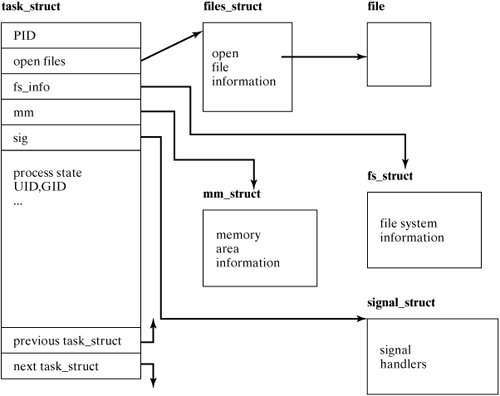
\includegraphics{task_struct.png}
    \end{center}
    
    \vspace{10mm}
    \begin{center}
        Figure \#2: Pid Hash Table (Glass, 555)
    \end{center}
    \begin{center}
        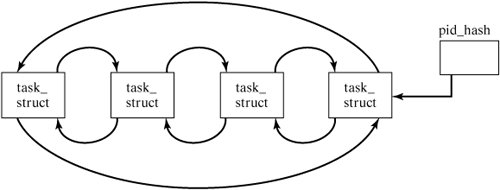
\includegraphics{pid_hash.png}
    \end{center}

\newpage
\begin{center}
    Example \#1: task\_struct Declaration
\end{center}
\begin{lstlisting}[frame=single]
struct task_struct {
/* these are hardcoded - don't touch */
  volatile long        state;          /* -1 unrunnable, 0 runnable, >0 stopped */
  long                 counter;
  long                 priority;
  unsigned             long signal;
  unsigned             long blocked;   /* bitmap of masked signals */
  unsigned             long flags;     /* per process flags, defined below */
  int errno;
  long                 debugreg[8];    /* Hardware debugging registers */
  struct exec_domain   *exec_domain;
/* various fields */
  struct linux_binfmt  *binfmt;
  struct task_struct   *next_task, *prev_task;
  struct task_struct   *next_run,  *prev_run;
  unsigned long        saved_kernel_stack;
  unsigned long        kernel_stack_page;
  int                  exit_code, exit_signal;
  /* ??? */
  unsigned long        personality;
  int                  dumpable:1;
  int                  did_exec:1;
  int                  pid;
  int                  pgrp;
  int                  tty_old_pgrp;
  int                  session;
  /* boolean value for session group leader */
  int                  leader;
  int                  groups[NGROUPS];
  /* 
   * pointers to (original) parent process, youngest child, younger sibling,
   * older sibling, respectively.  (p->father can be replaced with 
   * p->p_pptr->pid)
   */
  struct task_struct   *p_opptr, *p_pptr, *p_cptr, 
                       *p_ysptr, *p_osptr;
  struct wait_queue    *wait_chldexit;  
  unsigned short       uid,euid,suid,fsuid;
  unsigned short       gid,egid,sgid,fsgid;
  unsigned long        timeout, policy, rt_priority;
  unsigned long        it_real_value, it_prof_value, it_virt_value;
  unsigned long        it_real_incr, it_prof_incr, it_virt_incr;
  struct timer_list    real_timer;
  long                 utime, stime, cutime, cstime, start_time;
/* mm fault and swap info: this can arguably be seen as either
   mm-specific or thread-specific */
  unsigned long        min_flt, maj_flt, nswap, cmin_flt, cmaj_flt, cnswap;
  int swappable:1;
  unsigned long        swap_address;
  unsigned long        old_maj_flt;    /* old value of maj_flt */
  unsigned long        dec_flt;        /* page fault count of the last time */
  unsigned long        swap_cnt;       /* number of pages to swap on next pass */
/* limits */
  struct rlimit        rlim[RLIM_NLIMITS];
  unsigned short       used_math;
  char                 comm[16];
/* file system info */
  int                  link_count;
  struct tty_struct    *tty;           /* NULL if no tty */
/* ipc stuff */
  struct sem_undo      *semundo;
  struct sem_queue     *semsleeping;
/* ldt for this task - used by Wine.  If NULL, default_ldt is used */
  struct desc_struct *ldt;
/* tss for this task */
  struct thread_struct tss;
/* filesystem information */
  struct fs_struct     *fs;
/* open file information */
  struct files_struct  *files;
/* memory management info */
  struct mm_struct     *mm;
/* signal handlers */
  struct signal_struct *sig;
#ifdef __SMP__
  int                  processor;
  int                  last_processor;
  int                  lock_depth;     /* Lock depth. 
                                          We can context switch in and out
                                          of holding a syscall kernel lock... */  
#endif   
};
\end{lstlisting}

\newpage

    \ \\
    \textbf{Process Relationships}
    
    \ \\
    Unix splits process creation into two commands.  The first, fork(), makes a perfect copy of the calling process.  This copy, known as the child of the process that called fork().  Not surprisingly, the process that called fork() is known as the parent.  Since having an exact copy of the calling process is not useful in most cases, the child process frequently utilizes the exec system call.  The exec system call completely guts an existing process (this includes all code, heap data, and stack data) and replaces it with a new program specified in its arguments.  Some examples of this process are shown below.  For more information about the functions used in the example, consult the man pages listed later in this report.  
    
    \begin{center}
        Example \#2: Uses of fork/exec
    \end{center}
\begin{lstlisting}[frame=single]
#include<unistd.h>          (*@// Contains fork and exec@*)
#include<sys/types.h>       (*@// Contains pid\_t datatype@*)
#include<sys/wait.h>        (*@// Contains wait \& waitpid@*)
#include<errno.h>           (*@// Contains errno@*)
#include<string.h>          (*@// Contains strerror@*)

int main(int argc, char **argv)
{
    pid_t pid = fork();
    
    if(pid == 0)
    {
        execl("/bin/ls", "/bin/ls", "-la", NULL);
    }
    else if(pid == -1)
    {
        cout << "[ERROR]: Fork failed: " << strerror(errno) << endl;
    }
    else
    {
        waitpid(pid, NULL, 0);
    }
    _exit(0);
}
\end{lstlisting}

\newpage

    \ \\
    When a UNIX/LINUX system starts up, two processes are initialized by the kernel.  The first, process 0, is known as the swapper.  As its name implies, it controls the scheduling of all processes on the system.  The second, process 1, is known as init.  Init is critical in the initialization of the system and starts many important routines (This includes the login shell).  Afterwards, all other new processes are created using fork and exec.  

\end{myindentpar}

\newpage
\noindent
{\large \underline{UNIX man Pages}:}

\begin{myindentpar}{5mm}

    One incredibly useful feature of UNIX operating systems that many new developers do not know about is the built in manual system.  Using the command 'man', you can access information about most aspects of the operating system from general commands all the way to system call APIs.  
    
    \ \\
    The structure of man pages in UNIX are organized into sections by number follows (Wikimedia Foundation):
    \begin{enumerate}
        \setlength\itemsep{-0.1em}
        
        \item General Commands
        \item System Calls
        \item Library Functions (Specifically, the C standard library)
        \item Special Files
        \item File Formats
        \item Games
        \item Miscellanea
        \item System Administration
        
    \end{enumerate}
    
    \ \\
    You may (or may not, that's fine too) find the following manual pages useful when creating this assignment.  Each one of these lines can be executed as a valid shell command to open a particular manual page.  Note, the number indicates the manual section that that function resides.  
    
    \begin{itemize}
        \setlength\itemsep{-0.1em}
    
        \item \code{man 3 exec}
        \item \code{man 2 fork}
        \item \code{man 2 chdir}
        \item \code{man 2 pipe}
        \item \code{man 2 dup}
        \item \code{man 2 wait}
     
    \end{itemize}

\end{myindentpar}

\newpage
\noindent
{\large \underline{Bibliography}:}

\ \\
{[} 1 {]} \hspace{1.2mm} Bovet, Daniel Pierce. \textit{Understanding the Linux Kernel: From I/O Ports to Process}
\hspace*{1cm} \textit{Management}. U.S.A: O'Reilly, 2003. Print.

\ \\
{[} 2 {]} \hspace{1.2mm} Glass, Graham. \textit{Linux for Programmers and Users}. Upper Saddle River, NJ: Pearson
\hspace*{1cm} Prentice Hall, 2006. Print.


\end{document}
